\RequirePackage{luatex85}
\documentclass{acmart}
\usepackage{tikz}
\usepackage{pgfplots}
\usepgfplotslibrary{external}
\tikzexternalize
\begin{document}
\title{}
\begin{abstract} \end{abstract}
\maketitle
\section{XXXXXXXXX}\subsection{X XXXXXXXXXX XXXXXXX}\subsection{XXXXXXXX XX XXXXXXXXXXXXXXXXX XXXX}\subsection{XXX XXXXXXXX}
\section{XXXXXX XXXXXXXXXX XXX XXXXXXXXX}\subsection{XXX XXXXXXXX XX XXXX XXXXX}
\section{XXX XXXXXXXXX XX X XXXXXXXX}\subsection{XXXXXXXXXXXXXXXX XXXXXXXXXXX XXX XXXXXXXXXX}
\subsection{XXXXXX XXXXXXXXXXXX XXXXXXXX}
\section{XXXXXXX XXXXXXXXXX}\subsection{XXXXXXXX XXXXXXXXXXXX XXXX XX XXXXX}\subsection{XXXXXXX XXXXXXX XX XXXXXXX}
\subsection{XXXXX XXXX XXXX XXXXXXXXXX}\subsection{XXXX XXXXXXXXXX XXXX XXXXXXXX XXXXXXXXXXXXXX}
\subsection{XXXXXXXXXXX XXX XXXXXXXXXXXXX}
\section{XXXXXXXXXX}\subsection{XXXXXXXXXXXXXXX}
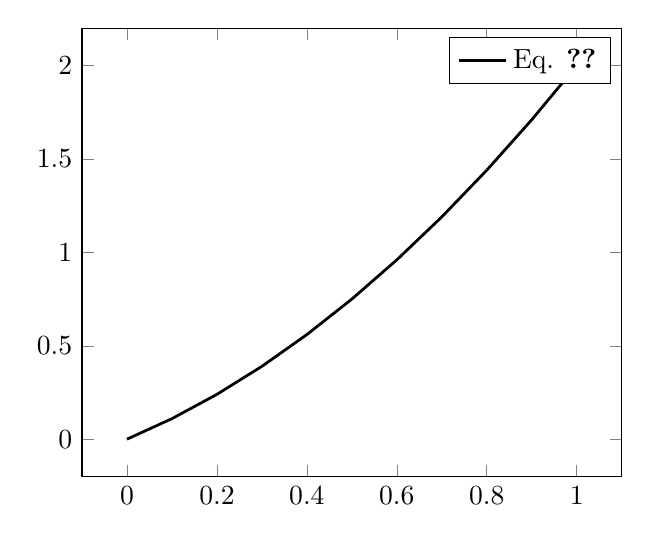
\begin{tikzpicture}
    \begin{axis}
      \addplot [color=black,solid,line width=1.0pt,domain=0:1,samples=11]{x+x^2};
      \addlegendentry{Eq. \ref{eq:equation}};
    \end{axis}
\end{tikzpicture}
\subsubsection{XXXXXXXXX XXXXXXXXXXXX}\subsubsection{XXXXXXXXXXX XXXXXXXXXXX XX XXXXXXXXXXXXXXX XXXXXXXXX}
\subsubsection{XXXXXXX XXX XXXXXXXXX XXXXXXXXX}\subsubsection{XXXX XXXXXXXXX}\subsection{XXXXXXXXXXXXXXX XXXX XXXXXXXXXXXX}
\section{XXXXXXX XXXX}
\section{XXXXXX XXXX}
\end{document}
